\chapter{Estudo preliminar}
\label{metodologia}

Nesse capítulo é apresentada uma comparação entre o Noosfero e os AVA, assim como a proposta de estudo desse trabalho para a minimização das diferenças entre o Noosfero e os ambientes virtuais de aprendizagem. É evidenciado a pesquisa que forneceu embasamento para direcionar o processo de desenvolvimento, inclusive a descrição das funcionalidades propostas e seus respectivos cenários de uso.

\section{Comparação entre Noosfero e ambientes virtuais de aprendizagem}
\label{comparacao-ava}

Como o objetivo do trabalho é a evolução de plataforma de redes sociais para um ambiente virtual de aprendizagem, a pesquisa realizada fundamenta-se no levantamento das principais funcionalidades que os AVA atuais utilizam, para verificar quais a plataforma o Noosfero ainda não possui. Desse modo surgiu a necessidade do levantamento das principais ferramentas AVA utilizadas atualmente pelas universidades e instituições de ensino, para proporcionar o mapeamento destas funcionalidades.
%
Os AVA selecionados para comparação são \textbf{BlackBoard}, \textbf{Sakai}, \textit{Modular Object-Oriented Dynamic Learning Environment} (\textbf{Moodle \footnote{Disponível em: \textit{ \url{https://moodle.org/}}}}) e \textit{TelEduc}.

O BlackBoard~\footnote{Disponível em: \url{http://www.blackboard.com/}}, é um dos maiores ambientes virtuais de aprendizagem utilizados atualmente por um, total de 72\% das TOP 200 melhores universidades do mundo \cite{blackboard}. Para utilização desta plataforma é necessário a aquisição de licenças por parte da instituição que pretende implementá-la. A plataforma tem total suporte da empresa que a mantém e não permite a modificação de sua estrutura interna pelos seus utilzadores. Os ajustes e melhorias de funcionalidades são realizados através do mapeamento dos comentários e sugestões dos usuários.

O Moodle, é um software livre criado em 2001 pelo educador cientista computacional Martin Dougiamas. É desenvolvido na linguagem de programação PHP e desta maneira pode ser instalado em qualquer sistema operacional que tenha suporte à linguagem. Para o seu uso podem ser utilizadas várias bases de dados com suporte a ODBC\footnote{Padrão para acesso a sistemas gerenciadores de bancos de dados}, tais como MySQL, PostgreSQL e Oracle.

O projeto Sakai\footnote{Disponível em: https://sakaiproject.org/ } ou a comunidade Sakai desenvolve e distribui o software livre Sakai como ambiente virtual de aprendizagem para colaboração e ensino para educadores, por educadores. A plataforma foi desenvolvido em linguagem Java e pode ser executado em várias plataformas diferentes como Linux, Unix, Windows e MAC. Suporta banco de dados MySQL e Oracle. As instituições que utilizam esta plataforma são abrangentes e estão listadas no site da comunidade \footnote{Disponível em: https://www.sakaiproject.org/community}.

O \textbf{TelEduc}\footnote{Disponível em: \url{http://www.teleduc.org.br/}} é um ambiente virtual de aprendizagem, cujo desenvolvimento iniciou em 1997, a partir de uma dissertação de mestrado de Alessandra de Dutra e Cerceau do Instituto de Computação da Universidade Estadual de Campinas\footnote{IC/UNICAMP. Disponível em: \url{http://www.ic.unicamp.br/}}. Foi objeto de pesquisa e desenvolvimento de um projeto coordenado pela Profa Dra Heloísa Vieira da Rocha\footnote{\url{http://lattes.cnpq.br/6985892121344767}} até 2012. Desde então, o projeto vem sendo evoluído para implementar ajustes e novas funcionalidades segundo \cite{rocha2002ambiente}, visando implementar necessidades relatadas por seus Usuários. O projeto é mantido pelo Núcleo de Informática Aplicada à Educação \footnote{NIED/UNICAMP. Disponível em:\url{http://www.nied.unicamp.br/}} da UNICAMP.

O TelEduc é um software livre desenvolvido na linguagem de programação PHP \footnote{Disponível em: \url{http://php.net/}} e JavaScript com banco de dados o MySQL \footnote{Disponível em: \url{https://www.mysql.com/}} para ambientes Linux. Em seu lançamento tornou-se um dos softwares mais utilizados para apoiar a educação à distância nas mais diversas áreas. Seus principais usuários são as universidades públicas e privadas, que utilizam a ferramenta para atividades educacionais, disponibilizando materiais, dando suporte a comunicação e interação entre os participantes.

Foram criadas tabelas comparativas (Tabelas \ref{tab:conteudo-atribuicao}, \ref{tab:curso}, \ref{tab:ferramentas}, \ref{tab:teste}, \ref{tab:permissoes-principal}) entre as ferramentas selecionadas e a plataforma Noosfero, desse modo fica mais evidente identificar quais funcionalidades a plataforma Noosfero carece. E vale ressaltar que não é objetivo deste trabalho esclarecer ou afirmar qual é a melhor ferramenta, mas verificar as principais funcionalidades dos AVA que são utilizados e aceitos pelas universidades.

As funcionalidades incluídas nas tabelas foram obtidas da literatura apresentada na seção \ref{ava}, e em uso aos ambientes onlines de demonstração, contando ainda, com o auxílio de mecanismos de ajuda fornecidos pelas ferramentas. Assim sendo, as funcionalidades selecionadas foram divididas em oito categorias:
\begin{itemize}
\item \textbf{Conteúdo:} relacionadas à criação e manutenção de conteúdos publicados pelos usuários.
\item \textbf{Atribuição:} permitem que os usários carreguem arquivos do seu computador local para a plataforma.
\item \textbf{Ferramentas:} mecanismos de apoio ao gerenciamento do conteúdo e ambiente;
\item \textbf{Teste/Quiz:} permitem a realização de avaliações e acompanhamento de resultados dos alunos;
\item \textbf{Comunicação:} possibilitam a comunicação síncrona e assíncrona entre os participantes de um curso;
\item \textbf{Curso:} fundamentais para organização dos cursos;
\item \textbf{Permissão e papéis:} utilizadas para gerenciar o ambiente, definindo papéis e autorizações de acesso ao ambiente;
\item \textbf{Página principal:} são as principais funcionalidades evidenciadas na página inicial de cada usuário.
\end{itemize}

Das categorias listadas na Tabela \ref{tab:conteudo-atribuicao}, podemos destacar que o Noosfero carece do SCORM \footnote{Um modelo de referência seja, conjunto unificado de especificações para a disponibilização de conteúdos e serviços de e-learning \cite{de2006objetos}.} e IMS-Content-Package \footnote{Padrão que permite exportar o conteúdo de um sistema de gerenciamento de conteúdo de aprendizagem ou repositório digital.} que são funcionalidades importantes para os AVA, pois permitem a importação de conteúdos de outras ferramentas proporcionando flexibilidade para o usuário.

Verifica-se que o Noosfero possui funcionalidades básicas de comunicação, mas não possibilita a comunicação síncrona (Bate-papo). Possui ainda, fórums que normalmente são utilizados para a divulgação de notícias e dúvidas, entretanto, não permite a assinatura de tópicos para o recebimento de notificações.

Como o Noosfero não é um ambiente virtual de aprendizagem, é possível verificar na Tabela \ref{tab:teste} que ele não possibilita a criação de questões para obter a resposta de usuários. Também não conta com a funcionalidade que permita ao professor atribuir as notas e acompanhar a situação de cada aluno. O Noosfero possui um \textit{plugin} denominado \textit{Work Assignment} que permite aos usuários enviarem arquivos para o servidor mas não possibilita que o moderador estabeleça uma pontuação para os mesmos.

\begin{landscape}

\begin{table}[H]
	\centering
	\begin{tiny}
	\begin{tabular}{C{4cm}C{3.2cm}C{3.2cm}C{3.2cm}C{3.2cm}C{3.2cm}}
	\toprule
	\textbf{Funcionalidades\textbackslash Sistema} & \textbf{BlackBoard 9.1} & \textbf{Moodle} & \textbf{TelEduc} & \textbf{Sakai} & \textbf{Noosfero}\\
	\midrule
	\multicolumn{6}{c}{\textbf{Conteúdo}}\\
	\midrule
	Diretórios/Pastas & Sim & Sim & Sim & Sim & Sim \\
	Criar/Extrair arquivos de pastas & Sim & Sim & Sim & Sim & Sim \\
	Editor HTML & Sim & Sim & Sim & Sim & Sim \\
	Filtro de vários idiomas & Não & Sim & \textbf{Não} & \textbf{Não} & Sim \\
	Audio & Sim {\tiny (incorporado no plugin do QuickTime)} & Sim & \textbf{Não} & Sim &  \\
	Vídeo & Sim & Sim & \textbf{Não} & Sim & Sim \\
	SCORM & Sim & Sim & \textbf{Não} & Sim & \textbf{Não} \\
	IMS-Content-Package & Sim & Sim &  &  & \textbf{Não} \\
	\midrule
	\multicolumn{6}{c}{\textbf{Atribuição}}\\
	\midrule
	Upload de um arquivo & Sim & Sim & Sim & Sim & Sim \\
	Upload de vários arquivos & Sim & Sim & \textbf{Não} & Sim & Sim \\
	Texto online & Sim(quiz) & Sim & Sim & Sim & Sim \\
	\midrule
	\multicolumn{6}{c}{\textbf{Comunicação}}\\
	\midrule
	Enviar e-mail & Sim & Sim & Sim& Sim   & Sim    \\
	Enviar mensagens& Sim & Sim & Sim& Sim   & Sim {\tiny(mural)}\\
	Bate papo& Sim & Sim & Sim& Sim   & \textbf{Não}    \\
	Fórum de discussão& Sim & Sim & Sim& Sim   & Sim    \\
	Alterar tipo de fórum & Sim & Sim & Sim& Sim   & Sim \\
	Fórum:   & Sim & Sim & Sim& Sim   & Sim    \\
	-postagem anônima & Sim & \textbf{Não} & \textbf{Não}& \textbf{Não}   & \textbf{Não}    \\
	-anexar um arquivo& Sim & Sim & \textbf{Não}& Sim   & \textbf{Não}    \\
	-os participantes podem criar tópicos   & Sim & Sim & \textbf{Não}& Sim   & Sim    \\
	-inscrever-se em um fórum  & Sim & Sim & \textbf{Não}& Sim   & \textbf{Não}    \\
	-assinar tópicos& Sim & \textbf{Não} & \textbf{Não}& Sim   & \textbf{Não}     \\
	-moderar fórum& Sim & \textbf{Não}  & Sim& Sim   & \textbf{Não}     \\
	Pesquisar fóruns& Sim & Sim & Sim& Sim   & Sim {\tiny (busca geral)} \\
	 & & & & & \\
	\bottomrule
	\end{tabular}
	\end{tiny}
	\caption{Tabela de comparação categorias: Conteúdo e Atribuição}
	\label{tab:conteudo-atribuicao}
\end{table}

\begin{table}[H]
	\centering
	\begin{tiny}
	\begin{tabular}{C{4cm}C{3.2cm}C{3.2cm}C{3.2cm}C{3.2cm}C{3.2cm}}
	\toprule
	\textbf{Funcionalidades\textbackslash Sistema} & \textbf{BlackBoard 9.1} & \textbf{Moodle} & \textbf{TelEduc} & \textbf{Sakai} & \textbf{Noosfero}\\
	\midrule
	\multicolumn{6}{c}{\textbf{Curso}}\\
	\midrule
	Criar cursos  & Sim & Sim & Sim  & Sim   & Sim    \\
	Criar novos papéis& Sim & Sim & \textbf{Não} & \textbf{Não}    & Sim \\
	Ferramentas de grupos & Sim & Sim & Sim& Sim   & Sim \\
	Relatórios do curso   & Sim & Sim & Sim& Sim   & \textbf{Não}  \\
	Sistema de alerta & Sim & \textbf{Não}  & \textbf{Não} & \textbf{Não}    & \textbf{Não}  \\
	Personalização ou configuração (nome, duração, inscrição, idioma) & Sim & Sim & Sim& Sim   & Sim    \\
	Formato de curso(fórum, formato dos tópicos, semanal)& \textbf{Não}  & Sim & \textbf{Não} &  & \textbf{Não}     \\
	Gerenciar campo menu  & Sim & Sim {\tiny O menu é personalizado de acordo com conteúdo o curso} & \textbf{Não} & Sim   & Sim    \\
	Customizar estilo de curso & Sim {\tiny (menu, tema)} & Sim {\tiny(tema) }& \textbf{Não} &  & Sim\\
	Estrutura de pastas   & Sim & Sim & \textbf{Não} & Sim   & Sim    \\
	Gerenciar ferramentas & Sim & Sim & Sim& Sim   & Sim    \\
	Backup do curso / exportação & Sim & Sim & \textbf{Não} & Sim   & Sim\\
	Importar curso& Sim & Sim & \textbf{Não} & \textbf{Não}    & \textbf{Não}  \\
	Restaurar curso & Sim & Sim & \textbf{Não} & \textbf{Não}    & \textbf{Não}     \\
	Importar conteúdo/características de outros cursos   & Sim & Sim & Sim & Sim   & Sim    \\
	Gerenciador de arquivos    & Sim & Sim & \textbf{Não} & Sim   & Sim \\
	\bottomrule
	\end{tabular}
	\end{tiny}
	\caption{Tabela de comparação categoria Curso}
	\label{tab:curso}
\end{table}

\begin{table}[H]
	\centering
	\begin{tiny}
	\begin{tabular}{C{4cm}C{3.2cm}C{3.2cm}C{3.2cm}C{3.2cm}C{3.2cm}}
	\toprule
	\textbf{Funcionalidades\textbackslash Sistema} & \textbf{BlackBoard 9.1} & \textbf{Moodle} & \textbf{TelEduc} & \textbf{Sakai} & \textbf{Noosfero}\\
	\midrule
	\multicolumn{6}{c}{\textbf{Ferramentas}}\\
	\midrule
	Glossário & Sim {\tiny (Editável pelo instrutor)} & Sim {\tiny (Os participantes também podem adicionar entradas) + bloco para glossário} & \textbf{Não}  & Sim & \textbf{Não} \\
	RSS Feeds & \textbf{Não}  & Sim {\tiny (Banco de dados, Fórum, Glossário)} & \textbf{Não}  & Sim & \textbf{Não}  \\
	Blogs & Sim & Sim & Sim & Sim & Sim \\
	Lista de contatos & Sim & Sim & Sim & \textbf{Não}  & Sim {\tiny (lista de participantes)}\\
	Calendário (Curso) & Sim & Sim & Sim & Sim & {\tiny Apenas de eventos} \\
	Permissões de acesso & Sim {\tiny (programada, dependendo de grau, dependendo do nível total do curso, depende do acesso a conteúdo definido, definir suas próprias regras)} & Sim \tiny{(programada, dependendo de grau, dependendo do nível total do curso, depende do acesso a conteúdo definidos / atividades)} & Sim & Sim & Sim \\
	Verificação de plágio & Sim {\tiny (integrado)} & \textbf{Não}  {\tiny (Não integrado, mas existem APIs)} & \textbf{Não}  & \textbf{Não}  & \textbf{Não}  \\
	Busca de arquivos (curso) & Sim {\tiny (adicionando um bloco correspondente)} & \textbf{Não}  & Sim & Sim & Sim \\
	Jornal & Sim & \textbf{Não}  & \textbf{Não}  &  & \textbf{Não}  \\
	Atividade concluída & Sim & Sim & Sim & Sim & Sim {\tiny (\textbf{Não}  totalmente implementado)} \\
	Ferramentas de voz & \textbf{Não}  (é necessário a ferramenta Wimba instalada) & \textbf{Não}  & \textbf{Não}  & Sim & \textbf{Não}  \\
	Permite o uso de módulos e plugins & Sim & Sim & \textbf{Não}  & Sim {\tiny (permite a seleção de ferramentas} & Sim \\ 
	\bottomrule
	\end{tabular}
	\end{tiny}
	\caption{Tabela de comparação categoria Ferramentas}
	\label{tab:ferramentas}
\end{table}

\begin{table}[H]
	\centering
	\begin{tiny}
	\begin{tabular}{C{4cm}C{3.2cm}C{3.2cm}C{3.2cm}C{3.2cm}C{3.2cm}}
	\toprule
	\textbf{Funcionalidades\textbackslash Sistema} & \textbf{BlackBoard 9.1} & \textbf{Moodle} & \textbf{TelEduc} & \textbf{Sakai} & \textbf{Noosfero}\\
	\midrule
	\multicolumn{6}{c}{\textbf{Teste/Quiz}}\\
	\midrule
	Banco de questões & Sim & Sim & Sim & Sim & \textbf{Não}  \\
	Exportar resultados & Sim & Sim & Sim & \textbf{Não}  & \textbf{Não}  \\
	Exportar respostas & Sim & \textbf{Não}  & \textbf{Não}  & Sim & \textbf{Não}  \\
	\textit{\textbf{Tipo de questões}} &  &  &  &  &  \\
	resposta com arquivo & Sim & Sim & \textbf{Não}  & Sim & Sim \\
	resposta por escala & Sim & Sim {\tiny (múltipla escolha)} & \textbf{Não}  & \textbf{Não}  & \textbf{Não}  \\
	preencher espaço vazio & Sim & Sim {\tiny (difícil de lidar)} & \textbf{Não}  & Sim & \textbf{Não}  \\
	múltipla escolha & Sim & Sim & Sim & Sim & \textbf{Não}  \\
	resposta múltipla & Sim & Sim & Sim & Sim & Sim {\tiny(permite o envio de várias versões de um arquivo)} \\
	Verdadeiro/Falso & Sim & Sim & Sim & Sim & \textbf{Não}  \\
	Calculos & Sim & Sim & \textbf{Não}  & Sim & \textbf{Não}  \\
	Resposta dissertativa & Sim & Sim & Sim & Sim & Sim {\tiny (com a creiação de um artigo)} \\
	Calculo numérico & Sim & Sim & \textbf{Não}  & Sim & \textbf{Não}  \\
	\bottomrule
	\end{tabular}
	\end{tiny}
	\caption{Tabela de comparação categoria Teste/Quiz}
	\label{tab:teste}
\end{table}

\begin{table}[H]
	\centering
	\begin{tiny}
	\begin{tabular}{C{4cm}C{3.2cm}C{3.2cm}C{3.2cm}C{3.2cm}C{3.2cm}}
	\toprule
	\textbf{Funcionalidades\textbackslash Sistema} & \textbf{BlackBoard 9.1} & \textbf{Moodle} & \textbf{TelEduc} & \textbf{Sakai} & \textbf{Noosfero}\\
	\midrule
	\multicolumn{6}{c}{\textbf{Permissões e papéis}}\\
	\midrule
	Papéis pré-definidos & Sim {\tiny (instrutor, assistente de ensino, construtor curso, nivelador, estudante, convidado;)} & Sim {\tiny (Administrador do site, gerente, criador do curso, professor editor, professor, estudante, convidado, usuário;)} & Sim {\tiny (coordenadores, formadores, alunos, visitantes, colaboradores;)} & Sim {\tiny (instrutores, assistente de professor, estudante;)} & Sim {\tiny (Administrador do sistema, moderador, membro, administrador de perfil;)} \\
	Editar papéis existentes & Sim & Sim & \textbf{Não}  & \textbf{Não}  & Sim {\tiny(apenas com permissão)} \\
	Criar novos papéis & Sim & Sim & \textbf{Não}  & \textbf{Não}  & Sim \\
	\midrule
	\multicolumn{6}{c}{\textbf{Página principal}}\\
	\midrule
	RSS Feeds & \textbf{Não}  & Sim & \textbf{Não}  & Sim & \textbf{Não}  \\
	Avisos/ Novos fóruns & Sim & Sim & Sim & Sim & \textbf{Não}  \\
	Lista de afazeres/ Próximos eventos & Sim & Sim & Sim {\tiny(Agenda)} & Sim & Sim {\tiny(Calendário)} \\
	Mensagens & \textbf{Não}  & Sim & Sim & Sim & Sim \\
	Boletim/ Resultados de questionários & Sim & Sim & Sim & Sim & \textbf{Não}  \\
	Usuários online & Sim & Sim & Sim & Sim {\tiny(chat)} & \textbf{Não}  \\
	Meu calendário & Sim & Sim & Sim & Sim & Sim \\
	Baixar o conteúdo completo do curso & \textbf{Não}  & \textbf{Não}  & Sim {\tiny(todos os arquivos)} & Sim & \textbf{Não}  \\
	Informação pessoal/ Perfil de usuários & Sim & Sim & Sim & Sim & Sim \\
	Cancelar a inscrição de um curso & Sim & Sim & \textbf{Não}  & Sim & Sim \\
	Software livre - GPL license & \textbf{Não}  & Sim & Sim & Sim & Sim \\
	Extensão a plataformas móveis & Sim & \textbf{Não}  & \textbf{Não}  & \textbf{Não}  & \textbf{Não}  \\ 
	\bottomrule
	\end{tabular}
	\end{tiny}
	\caption{Tabela de comparação categorias: Permissões e papéis, página principal}
	\label{tab:permissoes-principal}
\end{table}

\end{landscape}

Os AVA mencionados possuem papéis de usuários pré-estabelecidos (Tabela \ref{tab:permissoes-principal}), apesar do Noosfero possuir estes papéis preestabelecidos possui a vantagem de criação de papéis customizados, onde o administrador define quais as permissões para cada um deles.

O Noosfero carece de uma melhor estruturação dos conteúdos para o gerenciamento de um curso. Conforme evidenciado na Tabela \ref{tab:curso}, a plataforma não permite tratar os conteúdos na forma de cursos e tampouco a personalização de seus formatos (formato dos tópicos, duração). Além disso a ferramenta de calendário disponível mostra apenas as datas dos eventos criados, não disponibilizando aos alunos todas as atividades e duração do curso de forma limpa e organizada.

Quando analisados os itens da categoria de página principal (Tabela \ref{tab:permissoes-principal}) é verificado que o Noosfero necessita de um template próprio para cursos que reúne as informações principais dos alunos. Algumas dessas informações necessitam apenas de uma melhor disposição pela interface, como calendário e mensagens. Já outras exigem implementação como um sistema de avisos, usuários online e boletim.

Analisando todas as Tabelas elaboradas fica evidente que é essencial ao Noosfero um mecanismo para atribuição de notas e melhor controle sob o envio de tarefas. Esses são os pontos principais que regem um ambiente virtual de aprendizagem além das funcionalidades relatadas.

\section{Pesquisa com alunos}
\label{pesquisa-alunos}

Para melhor prosseguirmos com este trabalho, realizamos uma pesquisa junto aos alunos da FGA sobre o uso de redes sociais em seu dia a dia e sobre o seu uso para apoio as disciplinas cursadas na universidade. Para isso, foi criado um questionário com quatro questões de múltipla escolha, e para os itens associou-se a uma escala tipo \emph{Likert} de cinco pontos: Nunca; Raramente; Às vezes; Frequentemente; Sempre (Instruções de preenchimento no Apêndice \ref{apen-inst}). Com este tipo de escala, pode-se mapear todas as respostas seguindo a lógica em que há duas alternativas negativas, duas alternativas positivas e uma intermediária.

Nesta seção, apresentamos as questões elaboradas (Apêndice \ref{apen-quest}) e as respostas coletadas através da ferramenta \textit{Google Forms}. O questionário foi aplicado na rede social \textit{Facebook}, em grupos específicos da FGA. Foram coletadas, ao todo noventa e quatro respostas voluntárias ao questionário. Abaixo segue as questões com as respectivas análises de seus resultados, que estão representados graficamente no Apêndice \ref{apen-quest-result}.

\subsection*{Com que frequência você utiliza redes sociais?}

\begin{figure}[h]
    \centering
    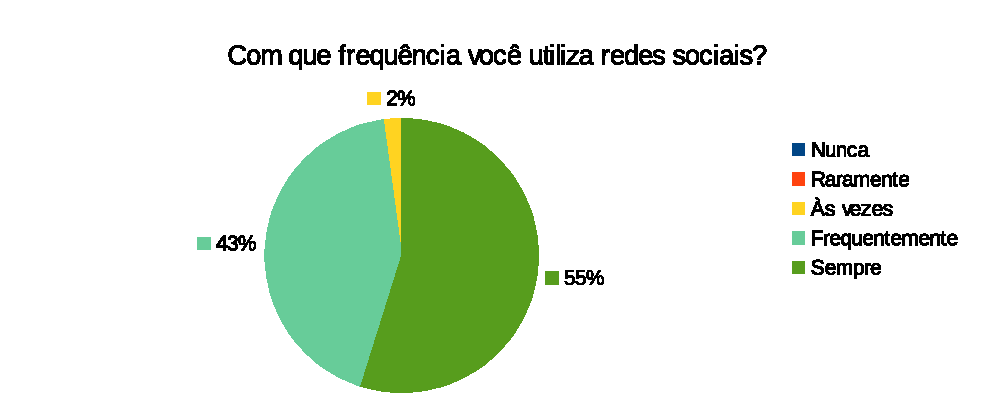
\includegraphics[keepaspectratio=true,scale=1]
      {figuras/pergunta1p.eps}
    \caption{Resultados do questionário para a pergunta \ref{pergunta1}}
    \label{fig:pergunta1}
\end{figure}

A primeira pergunta tinha como objetivo levantar com que frequência os alunos utilizam as redes sociais. Na Figura \ref{fig:pergunta1}, nota-se que 98\% dos alunos que responderam ao questionário utilizam as redes sociais sempre ou frequentemente, o que evidencia o fato que atualmente os estudantes dessa geração estão inseridos neste contexto.

\subsection*{Você utiliza alguma rede social como ferramenta de apoio as disciplinas?}

\begin{figure}[h]
    \centering
    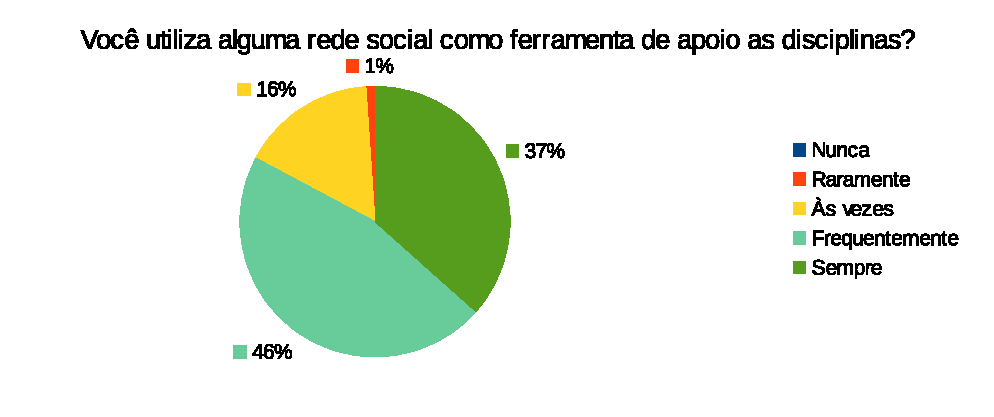
\includegraphics[keepaspectratio=true,scale=1]
      {figuras/pergunta2p.eps}
    \caption{Resultados do questionário para a pergunta \ref{pergunta2}}
    \label{fig:pergunta2}
\end{figure}

O intuito da segunda pergunta foi verificar se os alunos utilizam alguma ferramenta de redes social como ferramenta de apoio as disciplinas. Na Figura \ref{fig:pergunta2}, verifica-se que apenas 16\% dos alunos às vezes utilizam e de outro ponto de vista 83\% dos alunos fazem uso da rede para tal. Demonstrando que mesmo a universidade utilizando AVA os alunos se apoiam em redes sociais para discutir e compartilhar conteúdos referentes as disciplinas cursadas.

\subsection*{Os professores incentivam o uso de redes sociais para suas disciplinas?}
% 11\% Sempre
% 19\% frequentemente
% 52\% Ás vezes
% 17\% Raramente
% 1\% Nunca
\begin{figure}[h]
    \centering
    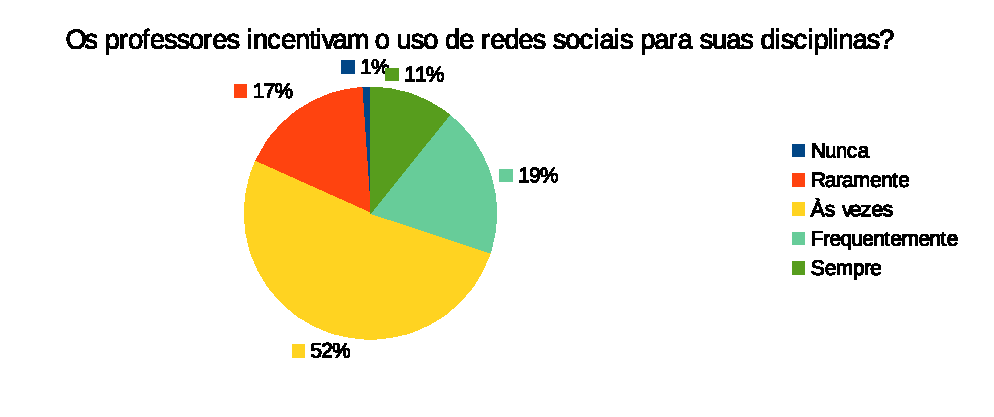
\includegraphics[keepaspectratio=true,scale=1]
      {figuras/pergunta3p.eps}
    \caption{Resultados do questionário para a pergunta \ref{pergunta3}}
    \label{fig:pergunta3}
\end{figure}

O objetivo desta pergunta foi verificar se mesmo que a universidade indique o uso de AVA se os professoes incentivam o uso das redes sociais em suas disciplinas. Na Figura \ref{fig:pergunta3}, percebe-se que pouco mais da metade dos alunos (52 \%) tem suas respostas em um ponto intermediário do questionário, mostrando que os professoes são bem imparciais quanto a isso. Apesar que do restante, tem-se mais respostas favoráveis do que contra.

\subsection*{Mesmo que o professor não recomende o uso de redes sociais para discussão de conteúdos de suas disciplinas, você as utiliza?}
% 30\% Sempre
% 45\% frequentemente
% 20\% Ás vezes
% 4\% Raramente
% 0\% Nunca
\begin{figure}[h]
    \centering
    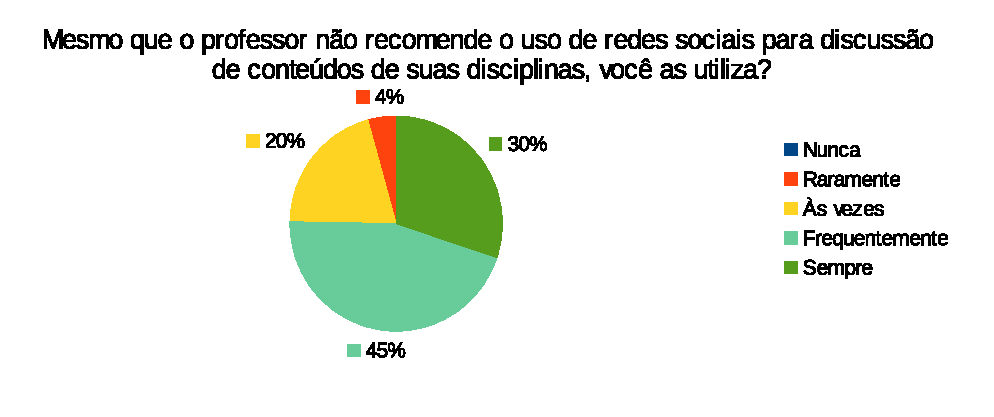
\includegraphics[keepaspectratio=true,scale=1]
      {figuras/pergunta4p.eps}
    \caption{Resultados do questionário para a pergunta \ref{pergunta4}}
    \label{fig:pergunta4}
\end{figure}

Na quarta e última pergunta buscou-se investigar se os alunos utilizam as redes sociais como uma ferramenta de apoio as disciplinhas mesmo que os professores não recomende seu uso para tal. Dos que responderam 75\% não levam em consideração tais recomendações e fazem o uso, demonstrando que os alunos preferem estar nas redes sociais onde expõem suas opiniões a fim de promover o compartilhamento de conteúdo (Resultados na Figura \ref{fig:pergunta4}).

Esta pesquisa exploratória mostra que mesmo com a existência de AVA os alunos utilizam as redes sociais, que não foram criadas com esse objetivo, para a discussão de assuntos relacionados ao ambiente acadêmico. Fundamentado nesses resultados e na comparação desses ambientes com o Noosfero, foram elaboradas funcionalidades para minimizar a diferença encontrada.

\section{Histórias de usuário}
\label{historia-usuario}

Nesta seção apresentaremos as funcionalidades desenvolvidas para contribuir para a adequação do Noosfero a um ambiente virtual de aprendizagem, para exercer a função de apoio aos AVA adotados pela Universidade. Serão apresentados os requisitos funcionais levantados para que esta possa suprir as necessidades levantadas.

A principais funcionalidades estão relacionadas ao \textit{plugin WorkAssignmnet}, além disso, julgou-se necessária a evolução do \textit{plugin Comunidade.UnB}. Este foi iniciado por \citeonline{bucher2013rede}, com objetivo de integrar o Noosfero com o serviço de Lightweight Directory Access Protocol (LDAP). Uma base LDAP é utilizada pela UnB para manter os dados de todos os seus alunos e funcionários.

As funcionalidades são apresentadas utilizando o utilizando o formato de histórias de usuários \footnote{Em inglês \textit{User Stories}(US)}, de acordo com as práticas ágeis. Além disso, os critérios de aceitação estão expostos no formato de cenários de uso, utilizando BDD.

\chapter{Histórias de usuário}
\label{apen-historia-usuario}
% história
\begin{description}

% ---------------------------------------------------------------------
\item [US01\label{us01}] \underline{Definir tempo restante}

\textbf{Como} um professor

\textbf{Gostaria de} definir o tempo restante para cada atividade no Work Assignment

\textbf{Para} gerenciar o envio de atividades pelos alunos em um determinado período.

\subsubsection*{Cenários de uso:}

\begin{enumerate}
\item \underline{Definir tempo}

\textbf{[Dado]} que esteja logado como professor

\textbf{[E]} selecione a o opção ``Gerenciar conteúdo''

\textbf{[Quando]} eu clicar em trabalho a ser entregue

\textbf{[Então]} devo visualizar a opção ``Ativar tempo de entrega''

\textbf{[E]} informar a data e hora máxima para envio da atividade.

\item \underline{Modificar tempo}

\textbf{[Dado]} que esteja logado como professor

\textbf{[E]} eu tenha atividades a ser entregue em aberto

\textbf{[E]} eu esteja visualizando as informações da atividade

\textbf{[Quando]} eu selecionar opção ``Editar''

\textbf{[E]} visualizar a opção ``Tempo de entrega''

\textbf{[Então]} deve ser permitido que eu altere o tempo definido

\textbf{[E]} visualize o resultado da alteração após a confirmação.

\item \underline{Permitir entrega de atividades após período}

\textbf{[Dado]} que esteja logado como professor

\textbf{[E]} selecione a o opção ``Gerenciar conteúdo''

\textbf{[E]} vavegar até a página trabalho a ser entregue

\textbf{[Quando]} selecionar a opção ``Ativar tempo de entrega''

\textbf{[Então]} devo visualizar a opção ``Permitir entrega após o período''

\textbf{[Para]} que eu possa selecioná-la.

\end{enumerate}

% -----------------------------------------------------------------------
\item [US02\label{us02}]\underline{Visualizar tempo restante de atividades}

\textbf{Como} um aluno

\textbf{Gostaria de} visualizar o tempo restante da atividade

\textbf{Para} enviar um arquivo na data correta.

\subsubsection*{Cenários de uso:}

\begin{enumerate}
\item \underline{Visualizar tempo}

\textbf{[Dado]} que esteja logado como Aluno

\textbf{[E]} eu esteja inscrito em um Curso

\textbf{[E possua atividade em aberto]}

\textbf{[Quando]} eu selecionar a opção de visualizar a atividade

\textbf{[Então]} eu devo visualizar se a atividade está em aberto

\textbf{[E]} qual o tempo restante para o envio da atividade.

\end{enumerate}

% -----------------------------------------------------------------------

\item [US03\label{us03}] \underline{Atribuir notas aos alunos}

\textbf{Como} um professor

\textbf{Gostaria de} atribuir notas as atividades enviadas pelos alunos

\textbf{Para} avaliar o rendimento de cada um deles.

\subsubsection*{Cenários de uso:}

\begin{enumerate}
\item \underline{Atribuir notas}

\textbf{[Dado]} que esteja logado como professor

\textbf{[E]} que a funcionalidade de notas esteja habilitada no plugin

\textbf{[Quando]} selecionar uma atividade na lista de atividades

\textbf{[Então]} devo visualizar a opção atribuir nota

\textbf{[E]} devo visualizar o campo ``nota'' para preenche-lo.


\item \underline{Alterar notas}

\textbf{[Dado]} que esteja logado como professor

\textbf{[E]} que a funcionalidade de notas esteja habilitada no plugin

\textbf{[Quando]} selecionar uma atividade na lista de atividades

\textbf{[E]} atividade já possua notas

\textbf{[Então]} devo visualizar a opção alterar nota

\textbf{[E]} devo visualizar o campo ``nota'' para preenche-lo.

\item \underline{Definir critério da nota final}

\textbf{[Dado]} que esteja logado como professor

\textbf{[E]} que a funcionalidade de notas esteja habilitada no plugin

\textbf{[Quando]} criar um trabalho a ser enviado

\textbf{[Então]} devo visualizar a opção de qual o critério para nota final

\textbf{[E]} devo selecionar qual a opção desejada.

\end{enumerate}

% -----------------------------------------------------------------------

\item [US04\label{us04}] \underline{Publicar notas aos alunos}

\textbf{Como} um professor

\textbf{Gostaria de} publicar as notas atribuídas as atividades

\textbf{Para} que os alunos possam visualizar suas respectivas avalizações

\subsubsection*{Cenários de uso:}

\begin{enumerate}
\item \underline{Disponibilizar notas de uma determinada atividade}

\textbf{[Dado]} que esteja logado como professor

\textbf{[E]} que a funcionalidade de notas esteja habilitada no plugin

\textbf{[Quando]} selecionar uma atividade na lista de atividades

\textbf{[Então]} devo visualizar a opção ``permitir visualização''

\textbf{[E]} devo ter a opção de ativá-lo.

\item \underline{Omitir notas de uma determinada atividade}

\textbf{[Dado]} que esteja logado como professor

\textbf{[E]} que a funcionalidade de notas esteja habilitada no plugin

\textbf{[Quando]} selecionar uma atividade na lista de atividades

\textbf{[Então]} devo visualizar a opção ``permitir visualização''

\textbf{[E]} devo ter a opção de desativá-lo.

\end{enumerate}

% -----------------------------------------------------------------------
\item [US05\label{us05}]\underline{Visualização das notas}

\textbf{Como} um aluno

\textbf{Gostaria de} visualizar minhas notas

\textbf{Para} inteira-me sobre minha pontuação nas atividades.

\subsubsection*{Cenários de uso:}
\begin{enumerate}

\item \underline{Visualizar cursos com notas disponíveis}

\textbf{[Dado]} que estou logado como ``Hebert''

\textbf{[E]} o plugin Work Assignment esteja ativo

\textbf{[E]} participo de alguma comunidade que utilize o plugin de notas

\textbf{[E]} existem notas de atividades disponíveis

\textbf{[E]} o professor tenha permitido sua visualização

\textbf{[Quando]} eu navegar até a página ``Minhas notas''

\textbf{[Então]} tenho que ver todos as comunidades (cursos) com notas disponíveis.

\item \underline{Detalhar notas de cada curso}

\textbf{[Dado]} que estou logado como ``Hebert''

\textbf{[E]} o plugin Work Assignment esteja ativo

\textbf{[E]} participo de alguma comunidade que utilize o plugin de notas

\textbf{[E]} existem notas de atividades disponíveis

\textbf{[E]} o professor tenha permitido sua visualização

\textbf{[E]} navegar até a página ``Minhas notas''

\textbf{[E]} visualizar todos as comunidades (cursos) com notas disponíveis

\textbf{[Quando]} eu selecionar a ``Visualizar detalhes'' de alguma comunidade

\textbf{[Então]} tenho que ver todos os grupos de atividades

\textbf{[E]} as notas disponibilizadas pelo professor.

\end{enumerate}

% -----------------------------------------------------------------------
\item [US06\label{us06}]\underline{Professor gerencia notas}

\textbf{Como} um professor

\textbf{Gostaria de} gerenciar as notas dos integrantes da comunidade

\textbf{Para} manter o controle sobre a pontuação de todos os alunos.

\subsubsection*{Cenários de uso:}

\begin{enumerate}

\item \underline{Definir grupo de atividades}

\textbf{[Dado]} que esteja logado como professor

\textbf{[E]} que a funcionalidade de notas esteja habilitada no plugin

\textbf{[E]} selecionar a opção ``Gerenciar notas''

\textbf{[E]} e eu selecionar o curso desejado

\textbf{[Quando]} eu clicar em ``Cadastrar grupo de atividades''

\textbf{[E]} eu preencho os campos \\
``Nome do grupo'',\\
e ``Lista de Atividades''\\
\textbf{[E]} eu clico em ``Salvar''

\textbf{[Então]} recebo uma mensagem de confirmação

\textbf{[E]} visualizo todas os grupos de atividades criados.

\item \underline{Visualizar notas de todos os alunos de uma determinada atividade}

\textbf{[Dado]} que esteja logado como professor

\textbf{[E]} que a funcionalidade de notas esteja habilitada no plugin

\textbf{[E]} selecionar a opção ``Gerenciar notas''

\textbf{[E]} e eu selecionar o curso desejado

\textbf{[Quando]} eu selecionar atividade

\textbf{[E]} algum aluno tenha enviado a atividade

\textbf{[Então]} devo visualizar todas as atvidades enviadas e suas respectivas notas.

\item \underline{Visualizar notas de todos ao alunos de um grupo de atividades}

\textbf{[Dado]} que esteja logado como professor

\textbf{[E]} que a funcionalidade de notas eteja habilitada no plugin

\textbf{[E]} selecionar a opção ``Gerenciar notas''

\textbf{[E]} e eu selecionar o curso desejado

\textbf{[Quando]} eu clicar em ``Visualizar notas por grupo de atividades''

\textbf{[E]} algum aluno tenha enviado a atividade

\textbf{[Então]} devo visualizar todas as atvidades daquele grupo e suas respectivas notas.

\end{enumerate}

% -----------------------------------------------------------------------

\item [US07\label{us07}] \underline{Bloco de notas recentes}

\textbf{Como} um aluno

\textbf{Gostaria de} visualizar minhas cinco últimas notas

\textbf{Para} facilitar a visualização do meu desempenho no curso.

\subsubsection*{Cenários de uso:}

\begin{enumerate}

\item \underline{Adicionar bloco}

\textbf{[Dado]} que esteja logado como aluno

\textbf{[Quando]} eu navegar até meu painel de controle

\textbf{[E]} eu selecionar a opção ``Editar Blocos Laterais''

\textbf{[E]} eu clicar na opção ``Adicionar bloco''

\textbf{[Então]} devo visualizar a opção ``Notas Recentes''

\textbf{[E]} devo ter a opção de adicioná-lo.

\item \underline{Visualizar cinco notas recentes}

\textbf{[Dado]} que esteja logado como aluno

\textbf{[E]} esteja com o bloco de notas recentes adicionado

\textbf{[E]} o professor tenha publicado alguma nota

\textbf{[Então]} devo visualizar o bloco com minhas cinco últimas notas

\textbf{[E]} o nome de cada atividade.

\end{enumerate}

% -----------------------------------------------------------------------

\item [US08\label{us08}] \underline{Bloco para visualização dos módulos}

\textbf{Como} um professor

\textbf{Gostaria de} visualizar um bloco com todos os módulos disponíveis no meu curso

\textbf{Para} facilitar a visualização da organização do curso criado.

\subsubsection*{Cenários de uso:}

\begin{enumerate}

\item \underline{Adicionar bloco}

\textbf{[Dado]} que esteja logado como professor

\textbf{[E]} e seja administrador da comunidade

\textbf{[Quando]} eu navegar até painel de controle da comunidade

\textbf{[E]} eu selecionar a opção ``Editar Blocos Laterais''

\textbf{[E]} eu clicar na opção ``Adicionar bloco''

\textbf{[Então]} devo visualizar a opção ``Lista de Grupos de trabalhos a serem enviados''

\textbf{[E]} devo ter a opção de adicioná-lo.

\item \underline{Editar numero de atividades listadas no bloco}

\textbf{[Dado]} que esteja logado como professor

\textbf{[E]} e seja administrador da comunidade

\textbf{[Quando]} eu navegar até painel de controle da comunidade

\textbf{[E]} eu selecionar a opção ``Editar Blocos Laterais''

\textbf{[E]} eu clicar na opção ``Editar bloco''

\textbf{[Então]} devo visualizar a opção ``Limite de trabalhos enviados''

\textbf{[E]} permitir escolher o número de itens a serem visualizados.

\item \underline{Visualizar módulos}

\textbf{[Dado]} que esteja logado como aluno

\textbf{[E]} seja membro da comunidade

\textbf{[E]} a comunidade possua grupos de atividades a serem enviadas

\textbf{[E]} possua trabalhos a serem enviados

\textbf{[Então]} devo visualizar o bloco todos os módulos disponíveis

\textbf{[E]} as atividades relacionadas a cada um deles.

\end{enumerate}

\item [US09\label{us09}]\underline{Autenticação via LDAP}

\textbf{Como} um aluno da Universidade Brasília

\textbf{Gostaria de} me autenticar na rede através da minha matrícula e senha

\textbf{Para} utilizar os mesmos dados de cadastro da UnB.

\subsubsection*{Cenários de uso:}

% cenário
\begin{enumerate}
\item \underline{Acesso sem matrícula cadastrada}

\textbf{[Dado]} que sou aluno da UnB

\textbf{[E]} possuo cadastro ativo na base de dados da UnB

\textbf{[E]} possuo cadastro ativo na base de dados do Comunidade.UnB

\textbf{[Quando]} eu acessar o portal

\textbf{Como} um aluno da Universidade Brasília

\textbf{[Então]} devo ser direcionado para uma página com o título ``Cadastrar Matrícula''

\textbf{[E]} devo ver os campos ``Matrícula'', ``Senha'' e
``confirmação de senha'' em branco.

\item \underline{Registro de matrícula de usuários existentes}

\textbf{[Dado]} que sou aluno da UnB

\textbf{[E]} me encontro na página de Cadastrar matrícula do Comunidade.UnB

\textbf{[Quando]} eu preencher os campos \\
``matrícula'' com ``100103979'',\\
e ``senha''  com a senha da base dados da UnB,\\
e ``confirmação de senha''

\textbf{[E]} clicar no botão ``Registrar''

\textbf{[Então]} eu devo ser direcionado para meu perfil
% cenários
\end{enumerate}

% historia
\end{description}

Neste capitulo foi apresentado as funcionalidades de um AVA em comparação com o Noosfero, bem como uma pesquisa realizada com os alunos para direcionar o desenvolvimento do trabalho. Este estudo é importante, uma vez que considerando esta análise, foi apresentado Seção \ref{historia-usuario} as funcionalidades que foram implementadas no desenvolvimento prático deste trabalho.
